Point-based methods learn features directly from the points and not from their spatial arrangement, as in projection-based methods. These methods differ in the architecture and on the basis of that they can be divided in pointwise MLP, convolution-based, graph-based and hierarchical data structure-based. In this survey we will present MLP, convolution-based and graph-based methods.

\subsubsection{Multi-Layer Perceptron}

In pointwise MLP methods, features from every point of a point cloud are extracted with independent Multi-Layer Perceptrons and then aggregated with a symmetric function, such as max pooling, in a unique vector that represents the whole point cloud; the process is illustrated in figure \ref{fig:mlp} (\cite{guo2020deep}). 

\begin{wrapfigure}{l}{0.4\textwidth}
    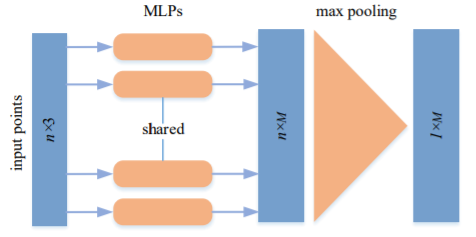
\includegraphics[width=1\linewidth]{images/mlp.png} 
    \caption{Architecture of PointNet.}
    \label{fig:mlp}
\end{wrapfigure}

\paragraph{PointNet}
\label{par:pointnet}

A famous architecture that uses MLP and directly consumes point clouds, without transforming them in other structures, is PointNet~\cite{qi2017pointnet}, one of the early attempts to design a deep network for consumption of unordered 3D point sets; this model is used for the task of classification as well as segmentation, in fact PointNet takes as input point clouds and outputs their class labels for the entire cloud (classification) or per point (segmentation). The transformations of data made by projection-based models render the data unnecessarily voluminous while introducing quantization artifacts, point clouds directly used, instead, are easier to learn from because of their simple and unified structures. Points in a point cloud are invariant to permutations, so they need at least a symmetrization to be fed into the networks.

A point cloud is a set of 3D points where each point is a three-dimensional vector, and can have other features such as color channels, that we don't consider. For the classification task the input point cloud is sampled from a shape or segmented from a scene, in this case the network outputs a score for each of the $k$ classes considered. For segmentation the input is a single object for region segmentation or a sub-volume of a scene, for this task the network outputs a score for each point and for each class.

A subset of points in an Euclidean space has three main properties: it is \textbf{unordered}, so the network that consumes $n$ points has to be invariant to $n!$ permutations of them; the points \textbf{interact} because they are immersed in a metric space and it has to be considered the distance between them and their neighborhood; the subset is \textbf{invariant under transformations} because rotating and translating points all together does not change the class the object belongs to.

\begin{figure}[ht]
    \centering
    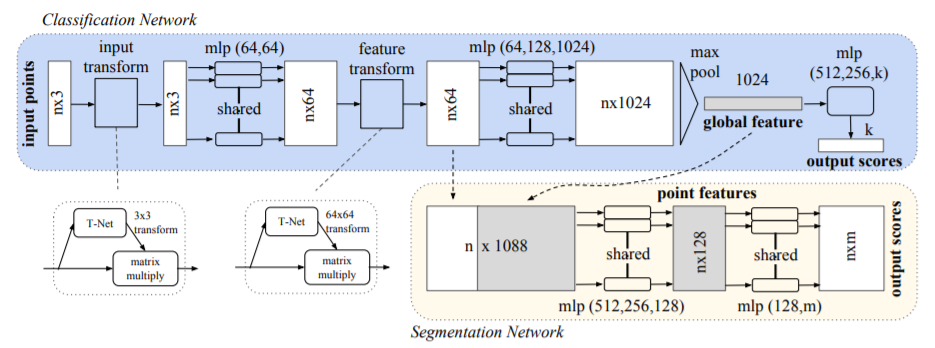
\includegraphics[width=\textwidth]{images/pointnet_architecture.png}
    \caption{Architectures of PointNet for classification and segmentation tasks.}
    \label{fig:pointnet_architecture}
\end{figure}

\paragraph{PointNet Architecture}

The input of the classification network of PointNet is a set of $n$ points ($n \times 3$ with 3 color channels), the network then applies a transformation of this set in many layers, as can be seen in figure \ref{fig:pointnet_architecture}, and then aggregates features with max pooling; the global feature tensor is then passed through another MLP that produces $k$ scores, one for every class.

\paragraph{Joint Alignment Network}

To achieve invariance to rigid geometric transformations, under which the predicted label for the point cloud must be preserved, a simple solution is to align all input set to a canonical space, instead in PointNet the T-net showed in figure \ref{fig:pointnet_architecture} is used: this mini-network is composed by point independent feature extractions, max pooling and fully connected layers. The T-net predicts an affine transformation matrix and applies it to the input points; another transformation matrix is applied later in the network, to the features space that has much many dimensions than the input space. The affine transformation matrices predicted by the T-net perform a \textit{pose normalization} to the point cloud, this also reduces the extent to which data augmentation is needed, because in point clouds the objects can take an infinite number of different poses. In order to improve optimization in such a big space, the matrix is constrained to be orthogonal by a regularization term added to the softmax training loss.

\paragraph{Symmetry Function for Unordered Input}

As previously said, the model has to be invariant to all points permutation, to achieve this objective PointNet uses a symmetric function that takes $n$ points and produces a new order-invariant vector. The idea on which is based the symmetric module of PointNet is that a generic function defined on an unordered set of points can be approximated by a function applied on the transformed points:

\[f(\{x_1, \dots ,x_n\}) \approx g(h(x_1), \dots , h(x_n))\]

where $f : 2^{\mathbb{R}^N} \to \mathbb{R}$, $h: \mathbb{R}^N \to \mathbb{R}^K$ and $g: \underbrace{\mathbb{R}^K \times \dots \times \mathbb{R}^K}_{n \text{ times}} \to \mathbb{R}$ is a symmetric function. In the network $h$ is a multi-layer perceptron and $g$ a composition of a single variable function and a max pooling function. Using a collection of $h$ the approximated $f$, $[f_1, \dots, f_K]$, are produced and they represent a global signature of the point set, invariant to points order. This method has a universal approximation ability proved with a theorem in \cite{qi2017pointnet}, that means that PointNet as a neural network is capable of approximate continuous set functions (as it is $f$); in the worst case, with this method the network will produce a volumetric representation of point clouds by partitioning the space in equal-size voxel, but in practice it learns a better strategy.

\paragraph{Theoretical Analysis}

In \cite{qi2017pointnet} the robustness of the network with respect to small perturbation of noise in points is proved: thanks to the architecture of the network and the chosen functions $h$ and $g$ defined above, for every set of points $S$ there exist two subsets $\mathcal{C}_S, \mathcal{N}_S \subseteq S$, such that for every set $T$, with $\mathcal{C}_S \subseteq T \subseteq \mathcal{N}_S$, it is true that $f(S) = f(T)$ and $|\mathcal{C}_S| \le K$, where $K$ is the dimension of the extracted features. In practice, $\mathcal{C}_S$ totally determines the output $f(S)$, for this reason it's called the \textit{critical point set} and its cardinality the \textit{bottleneck dimension of} $f$. This result shows that the extracted features from the point cloud remain unchanges if all the points of the critical point set are preserved and also with extra noise, up to $\mathcal{N}_S$, so PointNet is robust with respect to perturbation, corruption and extra noise points. In figure \ref{fig:critical_point_sets} critical point sets and upper-bound shapes for many objects are visualized.

\begin{figure}[ht]
    \centering
    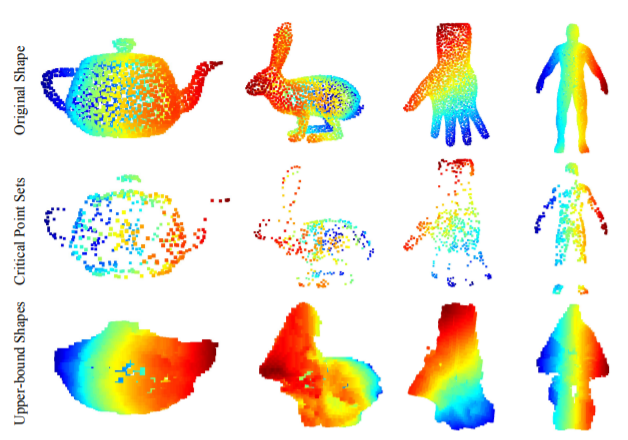
\includegraphics[width=0.5\textwidth]{images/critical_point_sets.png}
    \caption{Critical point sets and upper-bound shapes for unseen objects.}
    \label{fig:critical_point_sets}
\end{figure}

For the task of classification, the extracted global features are then passed through a simple MLP for output scores. For the task of segmentation, instead, the features pass through a new part of the network that's beyond the scope of this survey.

\paragraph{Results}

Validation experiments on PointNet has been made with dataset ModelNet40, described in this survey in \ref{subsec:datasets}; PointNet has been the first MLP network tested on ModelNet40. From the mesh faces 1024 points are sample uniformly and normalized in a unit sphere, then, during, training, these data are augmented with rotation and addition of Gaussian noise. The achieved mACC (section \ref{subsec:metrics}) is $86.2 \%$, while the O.A. is $89.2 \%$.

These results are achieved with the whole PointNet network, but other experiments have been conducted to demonstrate the effectiveness of input and features transformations (T-net). The performance difference with or without T-net are summarized in figure \ref{tab:t_net_accuracies}.

\begin{table}[ht]
    \centering
    \begin{tabular}{cc|l}
        \hline \text { \textbf{Transform} } & \text { \textbf{Accuracy} (\%) } & \text {\textbf{Description} }\\
        \hline none & 87.1 & no T-net applied \\
        \hline input (3x3) & 87.9 & T-net applied only to input points (3x1)\\
        feature (64x64)  & 86.9 & T-net applied only to features (64x1)\\
        feature (64x64) + reg. & 87.4 & T-net applied only to feature points and regularization on training loss\\
        \hline
        both & 89.2 & T-net applied to input points and features \\
        \hline
    \end{tabular}
    \caption{Effects of input feature transformations on PointNet performances.}
    \label{tab:t_net_accuracies}
\end{table}

To demonstrate robustness, the network has been tested in various kind of input corruption scenarios: with $50 \%$ of missing points from the input, the accuracy drops by $2.4 \%$. At last, the analysis of space and time: PointNet ha 3.5 millions parameters and has a computational cost of 440 millions FLOPs/sample (floating-point operations/sample); it's space and time complexity is linear in the number of input points so it is very scalable.

\paragraph{PointNet++}
\label{par:pointnet++}

PointNet is limited because it cannot capture local structures and fine geometric structures from the neighborhood of each point, so Qi et al. \cite{qi2017pointnet++} proposed a hierarchical network PointNet++, inspired by the fact that CNNs take features at different scales by a stack of convolutional layers.

PointNet learns a spatial encoding of each point and aggregates the points features in a global point cloud signature, but doing this it can't capture local structures induced by the metric of the space in which the point cloud is immersed. Using CNNs permits to progressively capture features at increasingly larger scales along a hierarchy and helps abstract local patterns to allow better generalization. PointNet++ has a \textit{local feature learner}, that is PointNet, that abstracts sets of points or local features, the weights of these local features are shared across the partitions, as in the convolutional setting. The partitions of the point cloud are overlapping local regions, defined as a neighborhood ball in the underlying Euclidean space.

\begin{figure}[ht]
    \centering
    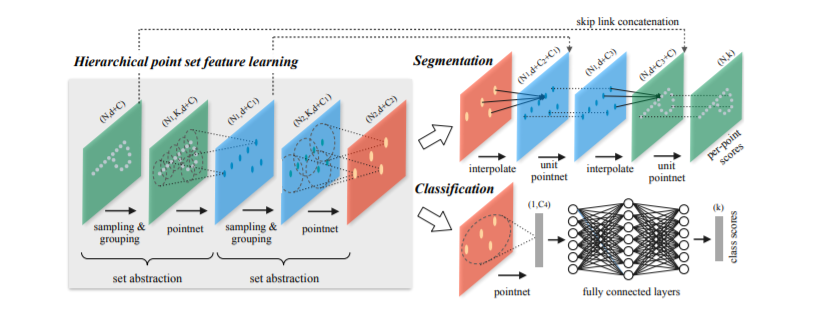
\includegraphics[width=\textwidth]{images/pointnet++_architecture.png}
    \caption{Architectures of PointNet++ for classification and segmentation tasks.}
    \label{fig:pointnet++_architecture}
\end{figure}

\paragraph{Hierarchical Point Set Feature Learning}

As it is shown in figure \ref{fig:pointnet++_architecture}, PointNet++'s structure is composed by set abstraction levels , in which the set of points is abstracted and a new smaller set is produced. Every set abstraction is composed of a \textit{Sampling}, a \textit{Grouping} and a \textit{PointNet} layer.

The Sampling layer selects a set of points from the input that will be the set of centroids of local regions; \textit{iterative farthest point sampling} (FPS) is used to choose the subset of centroids from the input set: a point is chosen to be a centroid if it's the most distant point, with respect to the metric, from the centroids previously chosen than the other points in the set. The Grouping layer builds local regions by computing the neighborhood of the centroids; the neighborhood of a centroid is built with all the points that are within a radius with respect to the metric distance (while in CNN the distance between pixels is defined by Manhattan's distance). Another way to construct centroids neighborhoods is k-NN search, but the first method guarantees a fixed region scale, making local region feature more generalizable across space. The \textit{PointNet layer} extracts feature vectors from the local regions; the input sets are the outputs of the Grouping layer, so they have different dimensions for every abstraction set, but PointNet is capable of extract fixed-length feature vectors from sets of different dimensions. Each local region is abstracted by a centroid and local feature that encodes the centroid's neighborhood, and the coordinates of points of a local region are first translated in a local frame relative to the centroid, in this way the network captures point-to-point relations in local regions.

\begin{wrapfigure}{l}{0.3\textwidth}
    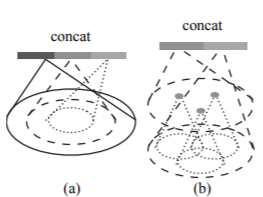
\includegraphics[width=1\linewidth]{images/density_adaptive_pointnet.png} 
    \caption{(a) Multi-scale grouping (MSG); (b) Multi-resolution grouping (MRG)}
    \label{fig:density_adaptive_pointnet}
\end{wrapfigure}

\paragraph{Robust Feature Learning under Non-Uniform Sampling Density}

The problem of non-uniform sampling density is faced in \cite{qi2017pointnet++}, in fact features learned in dense data may not be generalized in the case of sparse data available. In the case of low density areas it is not possible to inspect closely the point cloud, so larger scale patterns are looked for. To solve this problem, some \textit{density adaptive PointNet layers} are added to PointNet++ architecture, these layers learn to combine features from different scale regions when the density is different. So, instead of having a single scale for each abstraction level, as said above, in PointNet++ an abstraction level extracts multiple scales of local patterns and combines them intelligently according to local point density, this happens thanks to the density adaptive PointNet layers. 

There are two types of density adaptive layers: \textit{Multi-scale grouping} and \textit{Multi-resolution grouping}. MSG layers apply grouping layers with different scales followed by an application of PointNet to extract features at each scale, then features at different scales are concatenated to form a multi-scale feature vector; MSG approach is computationally expensive since it runs local PointNets at large scale neighborhoods for every centroid. MRG layers at every level $L_i$ build a concatenation of two vectors, the first one summarizes the features at every subregion from the previous features level in the network $L_{i-1}$ using the set abstraction level, the second one is obtained by processing all raw points in the local region at level $L_i$ with PointNet; when the density of a local region is low, the first vector is less reliable, but the second one is weighted higher, furthermore, when the density is high, the first vector have information of finer details.

\paragraph{Results}

PointNet++ has been evaluated on different datasets (2D objetcs, 3D objects, rigid and non-rigid objects,  real 3D scenes), including ModelNet40. All the point sets are normalized to be zero mean and within a unit ball, the architecture evaluated consists in a three-level hierarchical network with three fully connected layers. The overall accuracy achieved on ModelNet40 shape classification is $91,9 \%$.

\begin{figure}[ht]
    \centering
    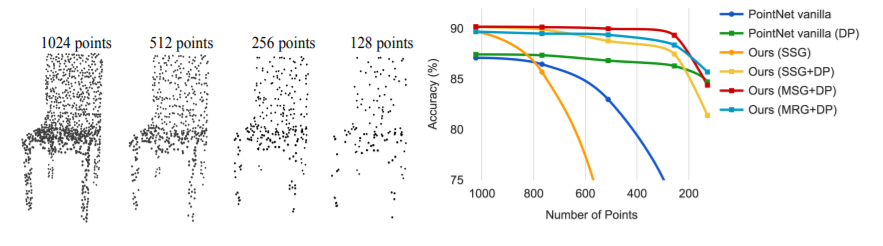
\includegraphics[width=0.8\textwidth]{images/pointnet++_density_robustness.png}
    \caption{Left: point cloud with random point dropout. Right: accuracy w.r.t. non-uniform density.}
    \label{fig:pointnet++_density_robustness}
\end{figure}

PointNet++ is more robust to density variations, in fact some points are randomly dropped during training to learn an optimized strategy to combine the multi-scale features. In figure \ref{fig:pointnet++_density_robustness} it is shown the robustness of PointNet++ with MSG or MRG, and DP (random dropout), with respect to PointNet.